\section{PyTorch Implementation} \label{sec:3-pytorch-impl}
In this section, I present my implementation of dynamic programming checkpointing with precise per-layer costs.
The implementation takes a sequence defined in PyTorch, profiles it, solves for the optimal policy, and executes the sequence according to the policy.
It is a standard Python 3 package that can be installed with \texttt{pip}.
However, I have not uploaded it to PyPI, so you must download the source and install it locally.
This is done as in Listing \ref{lst:3-install}.

\begin{listing}[h]
    \inputminted[
        frame=lines,
        framesep=2mm,
        baselinestretch=1.2,
        fontsize=\footnotesize,
        linenos,
        style=perldoc
    ]{bash}{listings/install_impl.sh}
    \caption{Installing the library.}
    \label{lst:3-install}
\end{listing}

%%%%%%%%%%%%%%%%%%%%%%%%%%%%%%%%%%%%%%%%%%%%%%%%%%%%%%%%%%%%%%%%%%%%%%%%%%%%%%%%
\subsection{Overview of API}
The library presents a helper class \texttt{SequentialCheckpointer}.
An overview of the API is given in Listing \ref{lst:3-demo}.
If the checkpointed sequence is not a sub-model of some larger model, meaning there are no more layers after it, then the upstream gradient given to the profiler and executor is simply 1 (recall that reverse-mode automatic differentiation is initialised with the gradient of the output with itself, which is 1).

\begin{listing}[h]
    \inputminted[
        frame=lines,
        framesep=2mm,
        baselinestretch=1.2,
        fontsize=\footnotesize,
        linenos,
        style=perldoc
    ]{python}{listings/impl_demo.py}
    \caption{Overview of the \texttt{SequentialCheckpointer} API.}
    \label{lst:3-demo}
\end{listing}

For greater flexibility, the profiling stage can be done separately to the policy solver stage.
Also, you can tell the solver to use uniform costs or to use given costs, shown in Listing \ref{lst:3-solve-with-costs}.
This can be done for both compute and memory, or only one.
Similarly, for flexibility, I have chosen to make the budget and policy not part of the class' state.
This way, the user can solve for many policies using the same profiling results.

\begin{listing}[h]
    \inputminted[
        frame=lines,
        framesep=2mm,
        baselinestretch=1.2,
        fontsize=\footnotesize,
        linenos,
        style=perldoc
    ]{python}{listings/solve_with_costs.py}
    \caption{Solving with uniform or given costs.}
    \label{lst:3-solve-with-costs}
\end{listing}

The API is very specific about where it expects input tensors to be in memory.
This is because the solver is very specific about what is in memory, in order to best utilise it.

If the last layer of an \(N\) layer sequence is the loss, then recall that \((b_{N+1}\) are the targets.
The solver expects this to be freed as the backwards pass proceeds.
Usually though, the user has a handle to the GPU copy of the tensors in the training loop, meaning the targets will not be freed.
Thus, the user must make a custom loss layer that moves the targets to the device only when needed.
This is trivial to do.
An example is given in Listing \ref{lst:3-loss-moves-targets}.

\begin{listing}[h]
    \inputminted[
        frame=lines,
        framesep=2mm,
        baselinestretch=1.2,
        fontsize=\footnotesize,
        linenos,
        style=perldoc
    ]{python}{listings/loss_moves_targets.py}
    \caption{A loss layer that moves the targets to the device.}
    \label{lst:3-loss-moves-targets}
\end{listing}

Secondly, the profiler expects the model to be on the device, but the inputs and upstream gradient to be on the CPU, so it can individually move layers to the device and profile them.
The model itself (which includes the parameter memory) will always be in memory during execution.
I choose to assume the user has already put the model on the device as it is common in PyTorch for users to move the model in-line as it is created, for example \texttt{create\_model().to(device)}.

On the other hand, the executor expects everything to already be on the device.
This is as it naturally should be though, as during the training loop everything will be on the device already.
Expecting them on the CPU would require the user to move them back to the CPU only for us to move it back.

Therefore, given the above, I do not think it is particularly ugly or paritcularly restrictive for the user to adhere to these assumptions.

%%%%%%%%%%%%%%%%%%%%%%%%%%%%%%%%%%%%%%%%%%%%%%%%%%%%%%%%%%%%%%%%%%%%%%%%%%%%%%%%
\subsection{Translating our Graph to PyTorch}
The computational graph of backpropagation derived in Section \ref{sec:2-4-2-peak-mem-training}, and the policy solver for it in Section \ref{sec:3-policy-solver} do not perfectly translate to PyTorch.
I provided them as they are to give a more generic approach that can be specialised to any framework, not just PyTorch.
The original computational graph is repeated here in Figure \ref{fig:2-simplified-comp-graph}.

\begin{figure}[h]
    \centering
    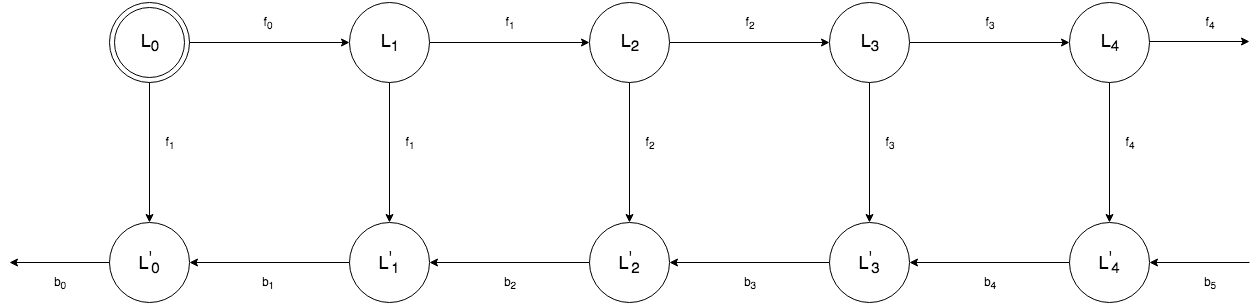
\includegraphics[width=0.9\linewidth]{simplified_comp_graph.png}
    \caption{The computational graph of backpropagation that we have defined checkpointing on.}
    \label{fig:3-simplified-comp-graph}
\end{figure}

Consider my definition of the backward operator \(L_k^\prime\).
It performs two operations: (i) computes the gradient of the parameters of the upstream layer using \(b_{k+1}\) and \(f_k\); and (ii) computes its downstream gradient using \(b_{k+1}\) and \(f_k\).
This means a backward operation computes its own downstream gradient, but the gradient with respect to its parameters is computed by the downstream layer.

This definition is not compatible with PyTorch.
A layer is a Torch module, which contains some parameters.
Running its forward function invokes an Autograd function on the parameters and the input to produce some output.
Thus, when the layer's backward function is called, it will call the backward function of the parameters too (as they require gradient).
It must be the case, then, that the layer's forward function saved its input as well as its output, as both are required to compute the gradient of the parameters.
This of course breaks the original graph, in which only the output of a layer goes to its backward function, meaning the assumptions baked into the policy solver about what memory is currently allocated do not hold.
Specifically, in PyTorch, the output of a layer \(f_k\), which feeds its backward function \(L_k^\prime\) to produce \(b_k\), will actually include the input \(f_{k-1}\) too.

To work around this, I simply redefine the forward tensors to include both the input and output, and the backward operators to compute the gradients of their own parameters.
The psuedo-tensor \(b_0\) is no longer required to represent the calculation of the first layer's parameters.
Instead, we now have \(N+1\) backward tensors, from \(b_1\) to \(b_{N+1}\).
As before, there are \(N+1\) forward tensors, from \(f_0\) to \(f_N\).

As this is what PyTorch is actually doing, redefining the forwards like this should not cause any major issues.
However, I have to amend the solver to be compatible with this.
The memory cost of computing the output of layer \(k\) is now just \(\beta^f_k\), not \(\beta^f_{k-1}\,+\,\beta^f_k\).
When we checkpoint \(f_k\) and recurse on the right, we are modelling that both the input and output have been checkpointed.
According to our original computational graph, this is suboptimal, but this is what PyTorch is doing, so I model it as such.
Changing this would require a fundamental change to Autograd.
Additionally, as the solver expects a \(b_0\), rather than change the solver, I simply pass in a dummy value with zero costs.

%%%%%%%%%%%%%%%%%%%%%%%%%%%%%%%%%%%%%%%%%%%%%%%%%%%%%%%%%%%%%%%%%%%%%%%%%%%%%%%%
\subsection{Imposing the Policy on a Network Through Autograd} \label{sec:3-pytorch-impl-autograd-recomp}
We need to be able to execute a sequence according to a given policy.
We can impose the dropping and recomputing of forwards in PyTorch through Autograd.

There is already a \texttt{torch.utils.CheckpointFunction} class in PyTorch.
It is an Autograd function that wraps the layer whose output should be recomputed.
In the forward function, it will save the input for the backward pass and run the layer with no grad, returning the output.
As the output was computed with no grad and was not saved for the backward pass, it will thus be freed.
In the backward function, the output is recomputed from the saved input, before running the backward function of the layer using the output.

We can use this function to encode `drops' into a list of layers.
That is, we create a \texttt{Drop} module that takes a child module and, in the forward, applies
\texttt{torch.utils.CheckpointFunction(child,\, x)} to implement recomputation.
We can then implement multiple recomputations by nesting \texttt{Drop} modules.
A \texttt{Drop} nested \(r\) times will have its forward called \(r+1\) times due to the \(r\) outer \texttt{Drop}s being recomputed, which invoke this \texttt{Drop}s forward again.
That is, the outer most \texttt{Drop}'s backward will recompute its child \texttt{Drop} and call its backward, which will recompute its child \texttt{Drop} and call its backward, and so on.
We would also need a \texttt{recursion\_depth} parameter.
We initialise it to \(r\), then every time the forward of \texttt{Drop} is called, it decrements \texttt{recursion\_depth} before invoking the checkpoint function. 
We amend \texttt{torch.utils.CheckpointFunction} to also take the \texttt{recursion\_depth} parameter and only save the input when this is 0.
This avoids the input being checkpointined repeatedly.

This solution allows the user to define a sequential model with \texttt{Drop}s encoded, run it normally, and \texttt{output.backward()} will handle all the recomputations naturally, as we have implemented the recomputation in Autograd.
The policy found by the solver can then be traversed to automatically encode the drops in the sequence for the user.
However, despite the elegance of this solution, it is actually fundamentally incompatible with our formulation of checkpointing.
The reason is that it checkpoints \textit{inputs} of layers and recomputes outputs, rather than checkpointing outputs, which is how the checkpointing policy was defined.

Consider, for a sequence \((i,\,j)\), the policy tells us to checkpoint \(k\).
We wrap the \(k^{\mathrm{th}}\) layer in a \texttt{Drop}.
We want to checkpoint its output \(f_k\).
Wrapping the \(k^{\mathrm{th}}\) layer means we actually checkpoint its input, \(f_{k-1}\).
This is not what was intended.
Say we instead wrap the \({k+1}^{\mathrm{th}}\) layer, we would checkpoint \(f_{k}\) correctly, but force \(f_{k+1}\) to be recomputed.
The problem is that by default forwards are kept in memory and \texttt{Drop} marks forwards to be dropped;
whereas the semantics of the policy solver is that all outputs are considered dropped unless the solver chooses to checkpoint them.

This fundamental difference could not be reconciled and meant that this approach had to be abandoned.

%%%%%%%%%%%%%%%%%%%%%%%%%%%%%%%%%%%%%%%%%%%%%%%%%%%%%%%%%%%%%%%%%%%%%%%%%%%%%%%%
\subsection{Manually Imposing the Policy on a Network}
Instead, we must create an executor function similar to the one used in Grusyls et al. \cite[Algorithm~2]{Gruslys2016} that manually checkpoints tensors and manually controls the backward pass, rather than leaving it to Autograd with \texttt{.backward()}.
The (adapted) psuedocode is given in Algorithm \ref{alg:3-ideal-executor}.

\begin{algorithm}[h]
    \DontPrintSemicolon
    \SetKwProg{Fn}{Function}{ is}{end}

    \SetKwFunction{ExecuteStrategy}{Execute\_Strategy}
    \SetKwFunction{ExecuteQuad}{Execute\_Strategy\_Quad}
    
    \SetKwFor{With}{with}{do}{end}
    
    \SetKwData{Torch}{torch}
    \SetKwFunction{NoGrad}{no\_grad}

    \SetKwData{True}{true}

    \Fn{\ExecuteStrategy{\(i,\; j,\; m,\; f_i,\; b_j,\; \beta,\; D\)}}{
        \BlankLine
        \tcp{Base Case}    
        \If{\(j \;=\; i\,+\,1\)}{
            run the backward operator of layer \(i\)\;
            \(b_i\;\leftarrow\; f_i\mathrm{.grad}\)\;
            \Return{\(b_i\)}
        }
        \BlankLine
        \(k\;\leftarrow\;D[i][j][m-1]\)\;
        \BlankLine
        \If{\(k\;=\;\)quadratic strategy}{
            \(b_i\;\leftarrow\;\) \ExecuteQuad{\(i,\; j,\; m,\; f_i,\; b_j,\; \beta\)}\;
        }
        \BlankLine
        \With{\Torch.\NoGrad{}}{
            \tcp{Run the forwards to k without gradient}
            \(f_k\;\leftarrow\;f_i\)\;
            \For{\(l \in [i+1,\, k]\)}{
                \(f_k\;\leftarrow\;\mathrm{Layer}_i(f_k)\)\;
            }
        }
        \BlankLine
        \(f_k.\mathrm{\_detach()}\)\;
        \(f_k\mathrm{.requires\_grad}\;\leftarrow\;\)\True\;
        \BlankLine
        \tcp{Recurse on the right and left}
        \(m_R\;\leftarrow\;m \;-\; \beta^f_k\)\;
        \(b_k\;\leftarrow\;\) \ExecuteStrategy{\(k,\; j,\; m_R,\; f_k,\; b_j,\; \beta,\; D\)}\;
        \(b_i\;\leftarrow\;\) \ExecuteStrategy{\(i,\; k,\; m,\; f_i,\; b_k,\; \beta,\; D\)}\;
        \BlankLine
        \Return{\(b_i\)}
    }

    \caption{Executes a network according to the given policy. Adapted from Grusyls et al. \cite[Algorithm~2]{Gruslys2016}. \texttt{Execute\_Strategy\_Quad} is not shown for brevity.}
    \label{alg:3-ideal-executor}
\end{algorithm}

The main PyTorch-specific consideration here is that we run the forwards to \(f_k\) with gradient tracking disabled, meaning the intermediate forwards will not be stored for the backwards pass.
We then re-enable gradients afterwards so following computations will be tracked.
We detach \(f_k\) because, otherwise, in the base case of the right subcall, when \texttt{.backward()} is called, it would attempt to propagate further back than layer \(k\).
We want to `interrupt' the backward pass at \(k\) so we can run the left hand side according to our policy.

However, this algorithm does not work.
There are a number of issues.

First, the stack frame of the current function holds a strong reference to \(b_j\) whilst the subcall proceeds right.
By the end of the subcall, we expect everything to the right of \(b_k\) to be freed, including \(b_j\).
However, the strong reference on our stack frame will prevent this.
The same problem happens when we recurse on the left.
I experimented with using Python's \texttt{weakref} library to hold only weak references from the stack frame of these recursive calls, so the only strong reference is from \(f_j\texttt{.grad}\).
However, this did not work as, for reasons as yet unknown, \texttt{weakref} did not count that reference so would deallocate the gradient tensor.

Also, the base case as written does not work.
Because of the above, the invariant is that \(f_i\) will be detached.
This means it will not have a backward graph though, so we cannot compute its backward.
Instead, we can remove that base case and instead have a \(j\,=\,i+2\) base case.
It computes the forward \(f_{i+1}\) before running the backward.
The recursive case now needs to manually check for the unit length base, and, if so, compute the forward and run the backward there, rather than recursing.

However, I unfortunately could not resolve the \texttt{weakref} problem.
I do have a simulator though.
Given a policy, it will simulate the execution according to the above algorithm and report back the total execution time and peak memory.
As we use precise profiled costs, these should be quite accurate.
